\documentclass[a4paper,oneside]{report}

\usepackage[utf8]{inputenc}
\usepackage[francais]{babel}
\usepackage[top=1cm, bottom=1.5cm, left=2cm, right=2cm]{geometry}
\usepackage{graphicx}
\usepackage{subfig}
\usepackage{titlesec}
%\usepackage{minted}
\usepackage[hidelinks]{hyperref}
\usepackage[backend=biber]{biblatex}
\usepackage{glossaries}

\addbibresource{rapport.bib}
\makeglossaries
% as a Service
\newacronym[
description={
Software as a Service. Modèle du Cloud Computing où l'on paye un abonnement pour utiliser un logiciel qui peut ne pas être présent physiquement sur notre ordinateur
}]{saas}{SaaS}{Software as a Service}

\newacronym[
description={
Platform as a Service. Modèle du Cloud Computing où un environnement d'exécution est mis à disposition du client pour ses propres applications
}]{paas}{PaaS}{Platform as a Service}

\newacronym[
description={
Infrastructure as a Service. Modèle du Cloud Computing où une infrastructure, potentiellement externe, est mis à disposition du client
}]{iaas}{IaaS}{Infrastructure as a Service}

% Services Amazon
\newacronym[
description={
Elastic Compute Cloud. IaaS d'Amazon
}]{ec2}{EC2}{Elastic Compute Cloud}

\newacronym[
description={
Elastic Block Store. Service de stockage bloc d'Amazon pour son IaaS, EC2
}]{ebs}{EBS}{Elastic Block Store}

\newacronym[
description={
Simple Storage Service. Service de stockage objet d'Amazon. Offre une stockage virtuellement illimité dans le cloud
}]{s3}{S3}{Simple Storage Service}

% HP
\newacronym[
description={
Integrated Lights-Out. Système de gestion \emph{out-of-band} d'HP pour ses serveurs
}]{ilo}{iLO}{Integrated Lights-Out}

\newglossaryentry{bladecenter}{
name = {BladeCenter},
description={Originellement nom donné à la gamme des serveur blades d'IBM. Désigne par extension tout les systèmes de serveur lames}
}

% Protocoles
\newacronym[
description={
Secure SHell. Protocole de communication sécurisé permettant le transfert de fichiers entre ordinateurs ou l'administration de serveurs à distance
}]{ssh}{SSH}{Secure SHell}

\newacronym[
description={
Lightweight Directory Access Protocol. Protocole de communication avec les annuaires respectant la norme du même nom. Généralement utilisé pour l'authentification des utilisateurs
}]{ldap}{LDAP}{Lightweight Directory Access Protocol}

\newacronym[
description={
Structured Query Language. Language permettant d'effectuer des requêtes sur des bases de données.
}]{sql}{SQL}{Structured Query Language}

\newacronym[
description={
Pluggable Authentication Modules. Système permettant d'intégrer différent schémas d'authentification à un système UNIX/Linux de façon transparente pour les applications
}]{pam}{PAM}{Pluggable Authentication Modules}

\newacronym[
description={
Network File System. Protocole qui permet d'accéder à des fichiers via le réseau
}]{nfs}{NFS}{Network File System}

\newglossaryentry{tunnelssh}{
name = {tunnel SSH},
description={Un tunnel SSH permet d'encapsuler le trafic IP dans une connexion SSH afin, par exemple, d'accéder à des machines distantes dont l'accès serait bloqué par un pare-feu}
}

\newglossaryentry{telnet}{
name = {Telnet},
description={Protocole permettant d'échanger très simplement des données entre deux ordinateurs}
}

\newacronym[
description={
Simple Network Monitoring Protocol. Protocole qui permet de gérer et de superviser des équipements réseaux
}]{snmp}{SNMP}{Simple Network Monitoring Protocol}

% Virtualisation
\newglossaryentry{virtualisation}{
name = {virtualisation},
description={En informatique, la virtualisation consiste à faire fonctionner plusieurs systèmes d'exploitations, ou plusieurs applications isolées les une des autres, sur un seul ordinateur}
}

\newglossaryentry{qemu}{
name = {QEMU},
description={Logiciel de virtualisation libre pour Linux}
}

\newacronym[
description={
Kernel-based Virtual Machine. Système de virtualisation libre basé sur QEMU et utilisant les extensions processeurs de virtualisation. Très performant et supporte tout les systèmes en tant qu'invités
}]{kvm}{KVM}{Kernel-based Virtual Machine}

\newacronym[
description={
LinuX Containers. Système de virtualisation léger intégré au noyau Linux qui permet de créer des environnements exécution isolés. Consomme très peu de ressources et très performant mais ne supporte que les systèmes Linux
}]{lxc}{LXC}{LinuX Containers}

\newglossaryentry{xen}{
name = {Xen},
description={Logiciel de virtualisation libre}
}

\newglossaryentry{hyperv}{
name = {Hyper-V},
description={Système de virtualisation de Microsoft présent dans Windows Server depuis la version 2008}
}

\newglossaryentry{vbox}{
name = {VirtualBox},
description={Logiciel de virtualisation de bureau développé par Oracle}
}

% Réseau
\newglossaryentry{switch}{
name = {switch},
plural = {switchs},
description={Équipement réseau de couche 2 permettant de connecter d'autres équipements entre eux}
}

\newacronym[
description={
Virtual LAN. Norme permettant d'isoler des réseaux à la couche 2 en utilisant la norme 801.1q afin d'ajouter un identifiant de réseau virtuel au début de la trame Ethernet
}]{vlan}{VLAN}{Virtual LAN}

\newacronym[
description={
Network Address Translation. Mécanisme permettant à des équipements possédant une IP privé de communiquer avec des hôtes situés sur un réseau publique
}]{nat}{NAT}{Network Address Translation}

\newacronym[
description={
Fibre Channel
}]{fc}{FC}{Fibre Channel}

\newglossaryentry{multipath}{
name = {Multipath},
description={Technique permettant d'utiliser plusieurs chemins physiques pour accéder à du stockage afin d'augmenter la bande passante et de fournir de la redondance}
}

\newacronym[
description={
Storage area network
}]{san}{SAN}{Storage area network}

\newglossaryentry{loadbalancing}{
name = {Load balancing},
description={Technique permettant de distribuer la charge sur plusieurs liens afin de maximiser la bande passante}
}

\newglossaryentry{failover}{
name = {Failover},
description={Technique consistant à basculer sur un autre équipement en cas de défaillance}
}

% Divers
\newacronym{api}{API}{Application Programming Interface}
\newacronym{crm}{CRM}{Customer Relationship Management}
\newacronym{kvmphys}{KVM}{Keyboard, Video, Mouse}

\newglossaryentry{raid0}{
name = {RAID 0},
description={Technique consistant à séparer les données}
}

\newglossaryentry{coeur}{
name = {coeur},
plural = {coeurs},
description={En informatique un coeur est une unité de calcul}
}

\newacronym[
description={Personal Package Archives. Dépôts non-officiel mise à disposition des développeurs de logiciel libre par la plateforme Launchpad
}]{ppa}{PPA}{Personal Package Archives}


% Frameworks
\newglossaryentry{cloudstack}{
name = {CloudStack},
description={Solution permettant de créer des IaaS créé par Citrix et Cloud.com}
}

\newglossaryentry{openstack}{
name = {OpenStack},
description={Solution permettant de créer des IaaS créé par Rackspace et la NASA}
}

% Sociétés
\newglossaryentry{rackspace}{
name = {Rackspace},
description={Hébergeur et fournisseur de solutions de Cloud Computing Américain. Créateur d'OpenStack}
}

\newglossaryentry{ovh}{
name = {OVH},
description={Hébergeur Français}
}

\newglossaryentry{sforce}{
name = {Salesforce},
description={Editeur de logiciel Américain très présent dans le domaine du Cloud Computing}
}

\newglossaryentry{dropbox}{
name = {Dropbox},
description={Service de stockage et de partage de fichiers en ligne}
}

\newglossaryentry{instagram}{
name = {Instagram},
description={Application de partage de photos pour iOS et Android}
}

\newglossaryentry{netflix}{
name = {Netflix},
description={Service de streaming de films sur Internet}
}

\newglossaryentry{shazam}{
name = {Shazam},
description={Logiciel de reconnaissance musicale}
}

% Clouds (voc)
\newglossaryentry{cloudcomputing}{
name = {Cloud Computing},
description={Désigne l'accès via un réseau à un ensemble de ressources informatiques partagées}
}

\newglossaryentry{cloudprive}{
name = {Cloud privé},
description={Infrastructure de virtualisation dont l'usage est réservé à une entreprise et qui le plus souvent géré et installé par celle-ci}
}

\newglossaryentry{cloudpublic}{
name = {Cloud public},
description={Infrastructure de virtualisation accessible publiquement moyennant éventuellement un paiement}
}

\newglossaryentry{stockagebloc}{
name = {stockage bloc},
description={Dans le cloud computing désigne le stockage qui est proche des disques physiques et qui offre de bonnes performances}
}

\newglossaryentry{stockageobjet}{
name = {stockage objet},
description={Dans le cloud computing désigne un type de stockage ne mettant pas l'accent sur la performance mais sur la facilité d'utilisation grâce à une API}
}

\newglossaryentry{glusterfs}{
name = {GlusterFS},
description={Système de fichiers distribués}
}

% Clouds publics
\newglossaryentry{gappengine}{
name = {Google App Engine},
description={PaaS de Google. Supporte Python, Java, et le Go}
}

\newglossaryentry{msazure}{
name = {Microsoft Azure},
description={IaaS et PaaS de Microsoft}
}

\newglossaryentry{sforcecloud}{
name = {Salesforce Sales Cloud},
description={Outil de CRM disponible via Internet}
}

\newglossaryentry{heroku}{
name = {Heroku},
description={PaaS de Salesforce. Supporte Ruby, Python, Java, Node.js, Clojure, et Scala}
}

\newglossaryentry{gapps}{
name = {Google Apps for Business},
description={Suite d'outils pour les entreprises (e-mails, agenda, bureautique) disponible via Internet}
}

% Licences
\newglossaryentry{opensource}{
name = {Open Source},
description={Terme s'appliquant aux logiciels dont la licence respecte la possibilité de libre de redistribution et d'accès au code source}
}

\newglossaryentry{licenceapache}{
name = {licence Apache},
description={Licence autorisant la modification et la redistribution du code tout en obligeant le maintien du copyright}
}

% Systèmes d'exploitation
\newglossaryentry{ubuntu}{
name = {Ubuntu},
description={Système d'exploitation libre soutenu par Canonical}
}

\newacronym[
description={Long Term Support. Pour Ubuntu signifie que le support est étendu à 5 ans contre 3 ans pour les versions standards
}]{lts}{LTS}{Long Term Support}


\newglossaryentry{windows}{
name = {Windows},
description={Système d'exploitation de Microsoft}
}

\newglossaryentry{windowsserver}{
name = {Windows Server},
description={Version serveur du système d'exploitation de Microsoft}
}

\newglossaryentry{linux}{
name = {Linux},
description={Système d'exploitation libre basé sur le noyau éponyme}
}

\newglossaryentry{solaris}{
name = {Solaris},
description={Système d'exploitation UNIX développé par Oracle}
}

\newglossaryentry{bsd}{
name = {*BSD},
description={Désigne une famille de systèmes d'exploitation dérivées d'UNIX}
}

% Languages de prog
\newglossaryentry{php}{
name = {PHP},
description={PHP: Hypertext Preprocessor. Langage de programmation principalement utilisé avec un serveur HTTP pour la création de sites et d'applications web.}
}

\newglossaryentry{java}{
name = {Java},
description={Langage de programmation orienté objet. Utilisé pour sa portabilité car la machine virtuelle Java (JVM) sur laquelle il est basé est disponible sur de nombreuses plateformes. D'après l'indice TIOBE, c'est le langage le plus populaire début 2013}
}

\newglossaryentry{ruby}{
name = {Ruby},
description={Langage de programmation orienté objet inspiré du Smalltalk et de Perl. Principalement connu pour la création d'applications web grâce au framework Rails}
}

\newglossaryentry{python}{
name = {Python},
description={Langage de programmation orienté objet}
}

\newglossaryentry{scala}{
name = {Scala},
description={Langage de programmation inspiré de Java}
}

\newglossaryentry{nodejs}{
name = {Node.js},
description={Logiciel basé sur la machine virtuelle JavaScript V8 de Google permettant d’exécuter du JS côté serveur et ainsi d'écrire des applications web scalables grâce, notamment, aux E/S asynchrones}
}

% Automatisation
\newglossaryentry{serviceorchestration}{
name = {service d'orchestration},
description={Programme qui permet d'automatiser la coordination et l'organisation de systèmes complexe}
}

\newglossaryentry{juju}{
name = {Juju},
description={Gestionnaire de paquet pour le cloud computing}
}

\newglossaryentry{puppet}{
name = {Puppet},
description={Logiciel permettant l'automatisation de la configuration de serveurs et de postes de travail écrit en Ruby}
}

\newglossaryentry{chef}{
name = {Chef},
description={Logiciel permettant l'automatisation de la configuration de serveurs et de postes de travail écrit en Ruby}
}

\newglossaryentry{cfengine}{
name = {CfEngine},
description={Logiciel permettant l'automatisation de la configuration de serveurs et de postes de travail écrit en C}
}

% Logiciels
\newglossaryentry{apache}{
name = {Apache},
description={Serveur HTTP. C'est le plus utilisé sur Internet}
}

\newglossaryentry{varnish}{
name = {Varnish},
description={Serveur de cache HTTP}
}

\newglossaryentry{mediawiki}{
name = {MediaWiki},
description={CMS permettant la création de Wiki}
}

\newglossaryentry{haproxy}{
name = {HAProxy},
description={Logiciel de répartition de charge}
}

\newglossaryentry{mysql}{
name = {MySQL},
description={Serveur de base de données}
}

\newglossaryentry{git}{
name = {Git},
description={Système de contrôle de versions distribué. Permet de partager et de synchroniser du code entre plusieurs développeurs}
}

\title{Rapport \\ \og Cloud privé avec OpenStack \fg}
\author{Julien Brun, Maxime Mouchet \\ Fréderic Pourraz (tuteur)}
\date{RT2 2012-13}

\titleformat{\chapter}[hang]{\bf\huge}{\thechapter}{2pc}{}

\begin{document}

\begin{figure}

\includegraphics[width=5cm]{images/iut.png}\hfill

\includegraphics[width=5.5cm]{images/rt.png}
\end{figure}

\maketitle

% La page vide après le titre
\clearpage
\thispagestyle{empty}
\null\newpage

\chapter*{Remerciements}
\thispagestyle{empty}
\noindent Nous remercions M. Frédéric Pourraz pour nous avoir permis de réaliser ce projet.\newline
\noindent Nous remercions M. Gaëtan Ferez pour nous avoir mis à disposition le matériel et son aide sur celui-ci.

\noindent De manière générale nous remercions tout les professeurs pour leurs enseignements durant ces deux années de DUT.

\renewcommand{\contentsname}{Sommaire}
\setcounter{tocdepth}{1}
\tableofcontents

\chapter{Introduction}
\section{Choix du sujet}
La \gls{virtualisation} et le \gls{cloudcomputing} sont des solutions d'avenir pour les entreprises grâce à des coûts réduits, une maintenance simplifiée, et une montée en charge aisée.
Nous trouvons ces technologies passionnantes et mettre en place un \gls{cloudprive} nous permet de les aborder tout en approfondissant les thématiques étudiées durant notre formation.

\section{Contexte}
\subsection{La \gls{virtualisation}}
Le principe de base de la \gls{virtualisation} est de permettre le fonctionnement de plusieurs \glspl{se} (\gls{windows}, \gls{linux}, …) en simultané sur un ordinateur.
Les intérêts sont multiples, on peut citer principalement :\newline

Augmenter la disponibilité grâce à une redondance et réduire les coûts.
Par exemple on peut imaginer avoir deux serveurs mails sur une même machine physique et utiliser l’un ou l’autre en fonction de leur charge ou en cas de panne.
On réduit par la même occasion les coûts puisqu’on n’utilisera qu’une seule machine physique pour ces deux serveurs.

Un dimensionnement plus facile. La \gls{virtualisation} ajoutant une couche d’abstraction entre le \gls{se} (logiciel) et le matériel (ordinateur) on peut aisément augmenter la puissance de calcul en ajoutant, par exemple, de la mémoire sur un ordinateur sans impacter le fonctionnement des systèmes virtuels.

Faciliter les migrations site-à-site.
Il est beaucoup plus facile de transférer un serveur d’un site physique à un autre en transférant une image virtuelle par le réseau plutôt qu’en transportant un serveur physique.\newline

Il existe plusieurs logiciels permettant de virtualiser des systèmes, parmi les plus connus on pourra citer \gls{vmwareesx} ou \gls{vbox}.

\subsection{Le \gls{cloudcomputing}}
\subsubsection{Vue d'ensemble}
Ces logiciels conviennent à la \gls{virtualisation} de quelques machines mais pas à la gestion global d'une infrastructure, ils se contentent de faire fonctionner plusieurs \glspl{se} sur un seul ordinateur.
Ils ne permettent pas d'utiliser des ressources et du stockage présents sur plusieurs ordinateurs depuis un lieu distant et par plusieurs personnes.

On va alors regrouper toutes ces ressources (stockage, ordinateurs, logiciels de \gls{virtualisation}) via un réseau.
On parle de \gls{cloudcomputing} et plus précisément\footnote{Voir \og IaaS, PaaS, et autres *aaS \fg ci-dessous.} dans ce cas là d’\gls{iaas}.
L'utilisateur final ne se préoccupe pas de savoir où est physiquement le stockage ou les ordinateurs qui possèdent le logiciel de \gls{virtualisation}, ni comment ils sont reliés entre eux. Il indique juste au cloud qu’il souhaite tant de machines avec tel système d'exploitation.

\subsubsection{IaaS, PaaS, et autres *aaS}
\glsreset{iaas}
Dans le domaine du \gls{cloudcomputing} il existe plusieurs niveaux d’abstractions, offrant des fonctionnalités plus ou moins haut niveau, on parle de modèles de services.
Leur nom prend la forme Sth- as a Service.

Les trois modèles les plus courants sont l'\gls{iaas}, le \gls{paas}, et le \gls{saas}.
Ce dernier représente le plus haut niveau d'abstraction.\newline
Dans ce modèle les clients paient un abonnement pour utiliser un logiciel dont ils n'auront pas à gérer l'installation et la maintenance.
Les applications courantes sont les \gls{crm}, la visioconférence, et les emails.
On peut citer pour exemple \gls{gapps} ou \gls{sforcecloud}.

Vient ensuite le \gls{paas}, où les applications fonctionnent également sur une plateforme externalisée (dans le Cloud) mais, à la différence du \gls{saas}, elles sont développés par le client.\newline
Cela permet aux entreprises de disposer d'un environnement d'exécution pour leur applications internes rapidement.
Par exemple, \gls{heroku}, le \gls{paas} de \gls{sforce} est capable d'exécuter de nombreux langages, tels que \gls{php}, \gls{ruby}, \gls{nodejs}, \gls{python}, \gls{java}, ou \gls{scala}.
On peut aussi citer \gls{gappengine} ou \gls{msazure}, qui offrent des fonctionnalités similaires.

Enfin vient l'\gls{iaas}, qui est le plus bas niveau d'abstraction. 
Ici le client dispose d'une infrastructure, mis à disposition par le fournisseur de Cloud, où il peut créer des serveurs virtuels à la demande, sans se préoccuper du matériel physique.
Il gère donc la configuration des systèmes d'exploitations et des logiciels qui s'y exécutent.

C'est ce dernier modèle que nous avons choisi d'étudier, nous allons donc détailler, dans la section suivante, les différentes solutions existantes avant de voir celle que nous avons retenu.

\subsubsection{Le stockage dans le cloud}
Dans le cas des \gls{iaas} on distingue deux types de stockages dans le cloud : le \gls{stockagebloc}, et le \gls{stockageobjet}.
Le premier est proche du matériel physique, limitant les couches d'abstractions, et offre des performances de haut-niveau.
Il est exposé aux instances virtuelles comme un disque physique natif, ce qui permet au système d'exploitation de démarrer dessus.\newline
Le \gls{stockageobjet}, au contraire, est dit \og haut-niveau \fg car il est accessible via une API et l'utilisateur final ne se préoccupe pas de savoir où, ni comment, ses données seront stockés.
Il est généralement plus lent que le \gls{stockagebloc} mais disponible en plus grande quantité et redondé, il est donc utilisé pour les données qui changent peu (images de machines virtuelles, sauvegardes, photos, ...).

\subsubsection{Cloud public vs. \gls{cloudprive}}
La différence majeure entre un Cloud dit \og public \fg, d'un Cloud dit \og privé \fg est le partage de l'infrastructure.
Dans le premier cas plusieurs clients se partagent l'infrastructure, tandis que dans le second seul une entreprise utilise l'infrastructure.\newline
Un Cloud public sera toujours situé en dehors de l'entreprise, alors qu'un \gls{cloudprive} pourra être installé dans l'entreprise et géré par elle-même.
Il en résulte alors un contrôle complet de l'infrastructure et une sécurité accrue.

\subsection{Panorama des IaaS}
\subsubsection{\gls{amazon} EC2}
\gls{amazon} a lancé \gls{ec2} durant l'été 2006.
Il s'agit d'un Cloud Public, au sens où l'infrastructure est commune à tout les clients, et accessible à travers une API et une interface Web, moyennant un paiement par heures d'utilisation.

Les instances, allant de 1 à 244Go de RAM et de 1 coeur virtuel à 32 coeurs physiques, sont virtualisés grâce à l'hyperviseur Open Source Xen.
\gls{ec2} supporte \gls{linux}, *BSD, Solaris, et \gls{windows} comme systèmes d'exploitations invités.

Le \gls{stockagebloc} est fourni par \gls{amazon} \gls{ebs} tandis que le \gls{stockageobjet} est fourni par \gls{amazon} \gls{s3}.
Chacun de ces service possède sa propre API, permettant de les utiliser indépendamment les uns des autres.

A titre informatif, \gls{ec2} est utilisé, entre autres, par \gls{netflix}\footnote{En 2011, aux heures de pointes, Netflix était responsable de 29\% du trafic Internet en Amérique du Nord \cite{NetflixTrafic}. D'où la nécessité d'une infrastructure robuste et scalable.}, \gls{instagram}, et \gls{shazam}, tandis que la plupart des services de stockage en ligne grand public, comme \gls{dropbox}, utilisent \gls{s3}.

Il faut noter que l'\gls{iaas} d'\gls{amazon} est propriétaire et spécifique à leur infrastructure. Il n'est pas possible de la déployer sur son propre matériel.

\subsubsection{OpenStack}

\subsubsection{CloudStack}
CloudStack est un système de création d'IaaS originellement développé par Cloud.com puis racheté par Citrix à l'été 2011.
Il appartient désormais à la fondation Apache et est donc Open Source sous la licence correspondante.\newline


\section{Rappel du cahier des charges}
\subsubsection{Objectifs}
Dans un premier temps nous voulions mettre en place un \gls{cloudprive} sous la forme d'une IaaS avec OpenStack.
L'objectif était de permettre à des utilisateurs (des élèves par exemple) de créer des machines virtuelles très rapidement même sur des machines disposant de peu de ressources.\\

Ensuite nous avons voulu mettre en place une solution pour automatiser la configuration des instances.
L'objectif était de permettre à un/des administrateur(s) de modifier une configuration ou de rajouter une application même après qu'une image ait été créé.

\subsubsection{Fonctionnalités à implémenter}
\begin{itemize}
\item Un noeud de \gls{virtualisation} avec \gls{kvm}
\item Authentification \& Autorisations avec un LDAP
\item Interface simple d'utilisation pour la création d'images
\item Personnalisation des instances au lancement suivant l'utilisateur (montage des disques, ...)
\end{itemize}

\subsubsection{Perspectives}
\begin{itemize}
\item Haute-disponibilité, tolérance de pannes
\item Monitoring des machines physiques
\item Nœuds de \gls{virtualisation} supplémentaires avec Xen, LXC, voir Hyper-V
\item Migration automatique des VMs après la chute d'un noeud
\end{itemize}

\section{Démarche}
Initialement notre projet devait comporter deux grandes étapes: la mise en place d'une installation de développement, et le déploiement sur un BladeCenter. Après cette dernière étape et discussion avec notre tuteur, nous avons décidé de modifier l'installation que nous avions réalisé sur le BladeCenter afin de maximiser les possibilités de virtualisation et de simplifier l'administration.\newline
Au final ce sont donc ces trois grandes étapes que nous détaillons dans le chapitre \ref{cha:miseenplace}.

De plus la majorité de notre travail a été effectué à deux en simultané DETAILLER CA-------------


\chapter{Matériel}

\section{Serveur dédié OVH}
Nous avons réalisé la première partie de notre projet sur un serveur dédié Kimsufi d'OVH.
Il était équipé d'un processeur 64 bits à 3,4Ghz avec les extensions VT-x (Intel Core i3), de 8Go de RAM, et de 2x1To de stockage en RAID 0.

Il s'agit de la configuration minimale pour faire fonctionner une installation de développement d'OpenStack.

\section{BladeCenter HP}
Une fois notre projet fonctionnel sur le serveur dédié nous avons déployé une nouvelle installation d'OpenStack sur quatre lames du BladeCenter dont dispose notre département au sein de l'IUT.

La configuration est cette fois-ci beaucoup plus intéressante et permet d'entrevoir les réelles possibilités du \gls{cloudcomputing}\footnote{Toutefois, bien que le BladeCenter possède une puissance importante, ses composants sont assez anciens et ne supportent pas les technologies de \gls{virtualisation} matérielle (VT-x, VT-d, AMD-V), ce qui limite le nombre de systèmes invités possibles.}.

\subsection{Configuration matérielle}
Nous disposions de trois lames équipés chacune de deux processeurs AMD Opteron 250 (2,4GHz / 64 bits) et de 4Go de RAM, ainsi que d'une lame équipé de deux Opteron 275 (2,2GHz / 64 bits) et de 8Go de RAM.\newline
Toutes les lames possèdent une carte Fibre Channel (FC) QLogic Q2312 pour le stockage.

\subsection{Stockage}
Les lames ne disposant pas de stockage intégré, ce dernier est assuré pas un SAN HP StorageWorks relié en FC.
Ce dernier fournit une couche d'abstraction au-dessus des disques durs et permet d'exposer plusieurs disques \og virtuels \fg à une lame au travers du contrôleur FC.

\subsection{Réseau}
Chaque lame possède deux liens à 1Gbit/s que nous avons agrégés afin d'obtenir une bande passante de 2Gbit/s entre elles.
Sauf sur une lame, faisant office de Routeur/NAT, connecté à 1Gbit/s au réseau de l'IUT et à 1Gbit/s aux autres lames.

La séparation des réseaux est permise par l'ajout de tag sur des trames Ethernet avec un numéro de VLAN (encapsulation 802.1Q).


\chapter{Systèmes d'exploitations hôtes}
\section{Ubuntu Server}

\section{CentOS}

\section{Solaris}

\subsection{Les zones}


\chapter{Logiciels}
\section{OpenStack}
Parmi ces différents solutions nous avons choisi d'utiliser OpenStack car c’est un projet Open source (le code source est disponibles gratuitement sur Internet) très actif.
Il peut être considérée comme mature pour une utilisation en production car il est utilisé entre autre par Rackspace (un très gros hébergeur et fournisseur de solutions de \gls{cloudcomputing} Américain), la NASA, et Intel.

\subsection{La fondation OpenStack}


\subsection{Les services}
OpenStack est constitué de différents services gérant chacun une composante spécifique de l'\gls{iaas}.
\subsubsection{Keystone}
Ce service est indispensable, il permet de coordonnée l'authentification et l'accès aux autres services.\newline
Il expose une \gls{api} HTTP(S) sur deux endpoints, un public sur le port 5000, permettant l'authentification des utilisateurs, et un autre dit privé sur le port 35357 permettant les tâches administratives tels que la gestion des utilisateurs et des terminaisons de services.
Il supporte différents backends pour l'authentification, certains permettant la persistance et l'édition des données comme \gls{sql} ou \gls{ldap}, d'autres en lecture-seule comme \gls{pam}.\newline

\subsubsection{Nova}
C'est le service qui va gérer les systèmes de \gls{virtualisation} (\gls{kvm}, \gls{xen}, ...).
Il est chargé de créer/démarrer/arrêter les machines, et de gérer les ressources physiques qui leurs sont allouées, ainsi que le stockage bloc si Cinder n'est pas utilisé, et le réseau si Quantum n'est pas utilisé.\newline
Il utilise Keystone pour l'authentification.


\subsubsection{Quantum}


\subsubsection{Cinder}
Depuis la version Folsom le \gls{stockagebloc} possède son propre service indépendant 



\subsubsection{Swift}
Swift est le système de \gls{stockageobjet}. 

Il supporte deux systèmes d'authentification, Swauth hérité de Rackspace, et Keystone.

\subsubsection{Glance}
Glance s'occupe des images virtuelles\footnote{Une image est le modèle d'après lequel serons créer les machines.}.
Il enregistre leur caractéristiques et leur emplacements de façon à ce que les autres services n'aient pas à s'en occuper.

Il utilise Keystone pour l'authentification et peut, en plus du système de fichier local, utiliser Swift pour stocker les images.

\subsubsection{Dashboard}
C'est l'interface graphique qui permet à l'utilisateur final de gérer ses instances virtuelles.

\section{Puppet}
Une fois la ou les machines virtualisées, il faut les configurer et installer des applications. On peut effectuer ces tâches à la main mais il existe des solutions libre comme Puppet, Chef ou encore CfEngine qui permettent d'automatiser ces configurations et de les appliquer simultanément sur plusieurs machines.
Nous utiliserons Puppet car elle possède une communauté très active et la syntaxe de ses scripts de configuration nous semble la plus clair.

Puppet utilise des recettes pour configurer les machines.
Nous avons choisi de les stocker sur un serveur git afin de mieux gérer les différentes révisions et l'édition distante.

\section{Reverse Proxy}
Nous avons décidé de ne connecter directement aucun service avec l'extérieur pour des raisons de sécurité, de contrainte technique (une seul ip disponible sur le réseau de l'IUT) et de facilité de mise en œuvre (configuration du pare-feu simplifié).
De cette manière, la zone qui abrite le dashboard n'est connecté qu'au LAN interne des lames.
De cette manière, il nous faut un moyen de rendre le dashboard accessible depuis l'extérieur. Nous avons choisi de mettre une place une mécanique de reverse proxy\footnote{Nous aurions pu décider de translater le port 80 (HTTP) sur l'ip de la zone abritant le serveur web, mais cette solution aurait été moins souple.
En effet, la translation ne nous autorise qu'une seul redirection alors que le reverse proxy se base sur les données HTTP et non le port. De cette manière, il nous permet de crée autant de sous domaine que l'on veux et de les rediriger vers n'importe quel ip et port.}.

Un reverse proxy est un serveur qui permet de réécrire les requêtes HTTP afin, par example, de cacher à l'utilisateur l'architecture interne du réseau.
Grâce à lui, nous pouvons rediriger les requêtes vers notre serveur web.
Un reverse proxy permet aussi de mettre en cache les ressources statique d'un site pour l'accélérer et soulager les serveurs web ou encore répartir la charge entre plusieurs serveurs.

Il existe plusieurs programme qui permette de faire du reverse proxy.
Le mieux, de par sa communauté, la finesse de ces règles, et ces performances est, à notre avis, Varnish\footnote{https://www.varnish-cache.org/}.
C'est un logiciel libre utilisé par example par Facebook. Cependant, nous n'avons pas pu l'utiliser pour les raisons détaillé dans la partie dédié.

Nous avons donc décidé d'utiliser Apache comme reverse proxy. Apache est le serveur web le plus utilisé\footnote{D'après le site netcraft.com, en Février 2013, Apache est utilisé par près de 55\% des sites actif. (IIS de Microsoft et Nginx sont eux à 12\%)} dans le monde, à l'heure actuel.
Il propose une fonction de reverse proxy grâce au module mod\_proxy. Sa configuration un peu moins fine que Varnish mais suffisante pour notre utilisation.

\section{Supervision}
Afin d'être sur qu'il n'y aucun problème à la fois sur le réseau et sur les machines, il existe des programmes appelé logiciel ou plateforme de supervision qui, en s'appuyant sur le protocole snmp, vérifie en continu le bon fonctionnement de tous les équipements réseaux et de tous les logiciels installé sur les machines.
Ils peuvent vérifier de la place restante sur les disques jusqu'à l'état des interfaces réseaux des switchs, en passant par le nombre de clients connecté à la base MySQL.
Lorsque un problème est détecté, une alerte est émise\footnote{Soit par mail, soit par sms... Tout dépend du logiciel de supervision et de sa configuration.}

Le marché de la supervision est à la fois occupé par de grand constructeur comme HP avec leur gamme OverView et par des logiciel libre comme Zabbix ou Nagios.
Nous avons choisi pour notre part d'utiliser Shinken\footnote{http://www.shinken-monitoring.org/}.
Il a l'avantage de s'installer facilement, d'être compatible avec Solaris\footnote{Shinken est écrit en python ce qui le rend disponible pour presque tous les systèmes.} et d'être compatible avec les plugins nagios et ainsi de bénéficier de son l'immense communauté.

\chapter{Mise en place} \label{cha:miseenplace}
\section{Installation de développement sur un serveur dédié}
Nous avons réalisé une première installation d'OpenStack et des services associés sur un serveur dédié afin d'étudier le fonctionnement global.
Dans cette section nous ne détaillerons que les configurations des systèmes d'exploitations, et pas l'installation d'OpenStack qui sera abordé dans la section suivante sur le BladeCenter.

\subsection{Environnement de test}

\section{Déploiement sur un BladeCenter avec Solaris}

Par souci de simplicité, nous avons décidé de donner un nom (hostname) à chaque lame afin de les différencier plus facilement.
Les nom sont donné dans le schémas global (Annexe \ref{sch:glob}).
Par la suite, lorsque nous parlerons d'une lame en particulier, nous l'appellerons par son nom.

\subsection{Installation des systèmes}
Nous avons choisi d'installer Solaris 11 sur Fuji, Iyo, et Tenjin, et CentOS 6 sur Raijin.
Pour plus d'informations sur ce choix voir \ref{sec:compatblade}.

\subsubsection{Démarrage de l'installateur}
L'installation des systèmes est classique à l'exception du multipath qui requiert un paramètre de boot spécial sur CentOS afin d'être détecté.
Au prompt boot de l'installateur il faut taper : linux mpath.\newline
Sur Solaris il n'y a rien à faire de spécial.

\subsubsection{Configuration du stockage}
Parler du multipath etc..

\subsubsection{Configuration du réseau}
Comme expliqué précédemment, les lames Iyo, Tenjin et Raijin sont connecté en 2Gbit/s (deux interface 1Gbit/s agrégé) dans un Vlan dédié et non-relié à l'extérieur.
Fuji, quand à elle, a une interface sur le réseau extérieur (réseau de IUT avec accès à internet) et l'autre dans le LAN inter-lames.
De cette manière, tous le trafic transite par elle et peut être redirigé suivant les règles du reverse proxy et du pare-feu. 

Afin de donner accès à internet au lames du réseau interne, nous avons mis en place une translation d'adresse sur Fuji (NAT).
Sur Solaris, le pare-feu par défaut est ipfilter. La configuration (donné en annexe \ref{conf:NAT}) permet de translater l'adresse locale (192.168.1.0/24) vers l'adresse public (10.102.75.190).

Maintenant que nos machine on accès à internet, il faut qu'on rende disponible depuis l'extérieur les interfaces web des différent services disponible (Le dashboard, le panel Shinken et l'interface de configuration de Puppet).
Pour réaliser cela, nous allons utiliser un reverse proxy (expliqué précédemment). Une fois apache installé, il faut ajouter au fichier de configuration d'apache (httpd.conf) les directive de l'annexe \ref{conf:apacheProxy}.
Celle-ci renvoie tous le trafic qui arrive à apache vers la machine qui a l'ip 192.168.1.3 et sur sont port 80.

\subsubsection{Environnement de travail}
Afin de rendre l'utilisation des machines plus agréable et plus facile à configurer, nous avons ajouté plusieurs programme et modifié plusieurs configuration.

Nous avons commencé par installer un gestionnaire de paquet.
Solaris possède sont propre gestionnaire de paquet que l'on peut appeler par la commande pkg. Seulement, il y a assez peu de paquet disponible.
Une communauté s'est alors créé autour du projet OpenCSW, un gestionnaire de paquet qui contient un très grand nombre\footnote{le projet OpenCSW propose 3675 paquet en février 2013} de paquet compilé pour Solaris.
Les paquets s'installent très facilement avec la commande pkgutils et les dépendances sont bien géré. Nous avons pu grâce à OpenCSW, installer de nombreux paquets comme Zsh, Apache ou encore Tmux\footnote{Tmux est un multiplexeur de terminaux
Il permet d'avoir plusieurs terminaux dans la même fenêtre (et donc sur la même connexion \gls{ssh} dans notre cas)} sans avoir à les compiler avec toutes leurs dépendances. 


Zsh


Pour pouvoir configurer nos différente machines, nous nous connectons à elle via le protocole \gls{ssh}. 
C'est un protocole de communication sécurisé qui permet d'avoir un terminal distant sur une machine.
Notre configuration réseau nous permet d'accéder depuis le réseau de l'IUT seulement à Fuji.
Nous nous connectons donc depuis notre ordinateur personnel sur Fuji puis de Fuji vers une autre machine du réseau local.
Il est aussi possible de faire des tunnel \gls{ssh} (voir \ref{tunnelingSsh})

\subsection{Installation des zones}

\subsection{Mise en place d'OpenStack}
\subsubsection{Préliminaires}

\subsubsection{Installation du service d'identité}

\subsubsection{Installation du service d'images}

\section{Déploiement sur un BladeCenter avec ...}


\chapter{Problèmes rencontrés}
\section{Compatibilité des systèmes d'exploitations sur le BladeCenter}
\label{sec:compatblade}
L'installation des systèmes d'exploitation sur les lames fût plus compliquée que prévu, étant donné la configuration bi-processeur et les cartes Fibre Channel.

Après de multiples installations infructueuses, un appel au support HP et la vérification des versions des firmwares nous sommes arrivés à la conclusion que les noyaux Linux récents ($ > 2.6 $) sont trop instables.

Sans que nous puissions fournir d'explications, CentOS, dans sa dernière version (6.3), fonctionne parfaitement sur la lame équipée d'Opteron 275, alors qu'aucun autre système Linux (Debian, Ubuntu, Suse) n'y fonctionne.
Il suffit de préciser linux text mpath au prompt boot de l'installateur.

Sur les autres lames nous avons installé Solaris 11 qui fonctionne parfaitement et supporte le multipath/boot on SAN nativement.

\section{Versions de librairies incompatible sur Solaris}
\label{sec:libsolaris}

\chapter{Conclusion}
Parler des versions pas stables (master) d'OpenStack

\appendix
\chapter{Installation des systèmes d'exploitations sur les lames}
Les lames du BladeCenter ne disposant pas de lecteur optique et l'accès physique n'étant pas toujours faisable, il est possible de réaliser l'installation des systèmes d'exploitation à distance.
Nous détaillerons ici les fonctionnalités intégrés aux lames permettant de les gérer à distance, ainsi que l'installation des différents systèmes que nous avons utilisés.\newline
Note: les installations détaillés sont spécifiques au BladeCenter et correspondent à la configuration minimum pour faire fonctionner OpenStack. Des documentations plus exhaustives sont disponibles sur les sites respectifs des OS.

\section{Systèmes d'exploitations supportés}
\subsubsection{Systèmes officiellement supportés}
D'après HP les systèmes d'exploitations supporté sur les lames BL35p sont:
\begin{itemize}
\item Red Hat Enterprise Linux (RHEL) 5
\item Suse Linux Enterprise Server (SLES) 10
\item VMware ESX 2.5.5
\item Solaris 10
\end{itemize}

\subsubsection{Systèmes que nous avons testés}
Après de multiples essais nous avons conclus que les systèmes suivants sont stables et supportent le multipath en natif sur les lames:
\begin{itemize}
\item Solaris 11
\item CentOS 6.3 (uniquement sur les lames à base d'Opteron 275)
\item VMware ESXi 4.1 (dernière version installable, les versions suivantes requièrent les extensions processeurs LAHF et SAHF)
\item Xen Cloud Platform 1.6
\end{itemize}

\section{Integrated Lights-Out}
Chaque lame possède un serveur de gestion intégré, \gls{ilo}, permettant de gérer l'alimentation (allumage, extinction, reset), de connecter des médias virtuels, et fournissant un \gls{kvmphys} dans le navigateur.
Les \gls{ilo} sont sur un réseau privé en 10.100.100.0/24 qui est accessible depuis un serveur TSE à l'adresse manap.rt.iut-acy.local (10.102.75.190).

\subsection{Connexion}
\subsubsection{Serveur TSE}
Le serveur TSE manap.rt.iut-acy.local est accessible depuis tout poste de l'IUT à l'adresse 10.102.75.190:3389. \gls{windows} XP,Vista,7 et 8 possèdent un client RDP nommé "Connexion Bureau à distance". Sur Linux on pourra utiliser Remmina qui intègre le tunneling SSH (voir paragraphe suivant).


Depuis l'extérieur (WiFi, maison) il est nécessaire d'utiliser le VPN\footnote{Le téléchargement et l'installation du client VPN sont détaillés sur vpn.univ-savoie.fr} mais, celui-ci bloquant les ports peu utilisés (pour des raisons de sécurité), il faut également mettre en place un \gls{tunnelssh}\footnote{NANANANNA}.
Pour ce faire il faut d'abord demander un accès à srv-dev.iut-acy.local à la DSI puis configurer son client \gls{ssh}.\newline
Sur \gls{windows} on utilisera Putty\footnote{Les instructions de configuration du \gls{tunnelssh} sous \gls{windows} sont disponibles à l'adresse https://w3.iut-acy.univ-savoie.fr/institutionnel/service-informatique/faq/tunnel-ssh/} tandis que sur Linux, à défaut de client gérant le tunneling comme Remmina, on utilisera la commande ssh comme suit pour mapper le port local 10389 sur le port 3389 du serveur TSE:
\label{tunnelingSsh}
\begin{verbatim}
ssh -L 10389:localhost:10.102.75.190:3389 login@srv-dev.iut-acy.local
\end{verbatim}
Il suffira alors d'indiquer l'adresse 127.0.0.1:10389 dans le client RDP pour se connecter.

Le serveur, fonctionnant sous \gls{windowsserver} 2003, possède Firefox comme navigateur Internet, et plusieurs autres logiciels utiles, comme le client VMWare vCenter pour la gestion d'ESXi.

\subsubsection{iLO}
Il suffit d'indiquer l'adresse IP correspondant à l'iLO de la lame dans le navigateur et d'entrer ses identifiants.
\newpage

\subsection{Principales fonctionnalités}
\subsubsection{Gestion de l'alimentation}
La section \emph{Virtual Power} de l'onglet \emph{Virtual Devices} indique l'état actuel de l'alimentation de la lame et propose six options:
\begin{description}
\item[Momentary Press:] Équivalent à un appui court sur le bouton Power de la lame.
Permet de démarrer ou d'arrêter proprement le système.
\item[Press and Hold:] Équivalent à un appui de cinq secondes sur le bouton Power de la lame.
Permet d'éteindre la lame si le système ne répond plus.
\item[Cold boot of system:] Coupe l'alimentation pendant six secondes puis allume la lame.
Permet aux condensateurs de se décharger et ainsi de résoudre certains problèmes matériels.
\item[Reset system:] Redémarre la lame.
\item[Manual Override for BL p-Class:] Force le mise sous tension de la lame sans tenir compte de la puissance électrique disponible.
Peut éteindre les autres serveurs présents dans le même rack.
\item[Automatically Power On Server:] Si \emph{Yes}, permet de remettre automatiquement sous tension la lame après une coupure de courant.
\end{description}

\subsubsection{Média virtuel}

\subsubsection{Console distante}

\section{Installation de CentOS}
\subsection{Média d'installation} \label{sec:installmediacentos}
On réalisera ici une installation par le réseau, plus rapide et permettant d'obtenir les dernières versions des paquets.
Les images ISOs peuvent être obtenus de plusieurs miroirs\footnote{La liste à jour de tout les mirroirs de CentOS est disponible à l'adresse http://www.centos.org/modules/tinycontent/index.php?id=30} mais on préférera celui de l'IN2P3, connecté directement au réseau RENATER et qui offre donc d'excellents débits (de l'ordre de la dizaine de Mo/s).\newline
On téléchargera l'image ISO netinstall à l'adresse suivante:
\begin{verbatim}
http://mirror.in2p3.fr/linux/CentOS/[version]/isos/{i386,x86_64}/
\end{verbatim}

\noindent Le dossier contenant l'image d'installation est quand à lui situé à l'adresse:
\begin{verbatim}
http://mirror.in2p3.fr/linux/CentOS/[version]/os/{i386,x86_64}/
\end{verbatim}

\noindent Par exemple pour CentOS 6.3 x64 les URLs sont:
\begin{verbatim}
http://mirror.in2p3.fr/linux/CentOS/6.3/isos/x86_64/CentOS-6.3-x86_64-netinstall.iso
http://mirror.in2p3.fr/linux/CentOS/6.3/os/x86_64/
\end{verbatim}


\subsection{Options de boot}
Afin qu'Anaconda, l'installateur de CentOS, détecte correctement les cartes FC et le multipath et que l'installation se fasse en mode texte, il est nécessaire d'entrer la ligne suivante au prompt boot (ECHAP pour y accèder à partir de la version 6) :
\begin{verbatim} linux mpath text \end{verbatim}

\subsection{Configuration générale}
\subsubsection{Langue et clavier}
On choisira la langue que l'on souhaite mais l'Anglais est préférable car les messages d'erreurs y sont souvent plus explicites et on évite les traductions hasardeuses.\newline
Pour le clavier choisir le layout correspondant. Pour les claviers AZERTY on peut utiliser le layout fr ou fr-latin9 (avec la touche Euro).

\subsubsection{Méthode d'installation}
Étant donné que l'on utilise l'image ISO netinstall il faut choisir "URL" au dialogue "Installation Method".
Le dialogue suivant demande de configurer la carte réseau.
Pour IPv4 on préferera configurer l'adresse en statique.
Bien que début 2013 l'IPv6 ne soit pas encore routé sur le réseau de l'IUT son support peut-être laissé activé en prévision du futur.
Dans ce cas DHCPV6 OU RA ?\newline
Si l'on souhaite aggréger plusieurs cartes réseaux, on n'en configurera qu'une seule pour l'instant et l'aggrégation sera réalisé une fois le système installé.\newline
Dans le dialogue demandant l'URL contenant l'image d'installation on rentrera celle indiquée dans la section \ref{sec:installmediacentos}

\subsubsection{VNC}
A partir de la version 5 de CentOS l'installateur propose d'effectuer l'installation via VNC afin de proposer un partitionnement personnaliser ou de modifier les paquets à installer.
Étant donné que l'on souhaite installer un système minimal sur du stockage vide on continuera l'installation en mode texte.

\subsubsection{Fuseau horaire}
Linux sera le seul système installer "en dur" sur la lame, on peut donc laisser l'horloge système en UTC\footnote{EXPLIQUER BLABLABLABLABLA}.
Attention à bien choisir le bon fuseau horaire afin que le passage à l'heure d'été se fasse correctement et que le timestamp des logs soit cohérent entre les machines.

\subsubsection{Mot de passe}
Rien de spécial ici, il faut juste choisir un mot de passe sûr. Des sites comme random.org\footnote{PARLER DE RANDOM ORG} permettent de générer des mots de passes aléatoires.

\subsubsection{Partitionnement}
On souhaite installer le système sur du stockage vierge, on choisira donc d'utiliser le disque entier.
Si plusieurs disques sont présents on sélectionnera uniquement celui où le système résidera.
On configurera plus tard le stockage supplémentaire nécessaire aux images et aux instance virtuelles.

\subsubsection{Installation et premier redémarrage}
Après le partitionnement l'installation se déroule toute seule et l'installateur demande de confirmer le redémarrage à la fin.
Il faut bien penser à déconnecter le lecteur virtuel dans iLO afin d'éviter de redémarrer sur l'installation.\newline
A partir de ce moment il est possible d'accéder à la machine en \gls{ssh}.

\section{Installation de Solaris}

\section{Installation de Xen Cloud Platform}

\section{Installation de VMWare ESXi}

\chapter{Diagrammes Réseau et schémas de principe}
\section{Les differant services d'OpenStack}
\noindent 1. L'utilisateur demande la création d'une ou plusieurs instance.\\
2. OpenStack se charge de les crées et retourne les informations pour y accéder à l'utilisateur\\
3. L'utilisateur peut utiliser son instance\\
L'utilisateur final ne peut accéder qu'au dashboard.
\begin{center}
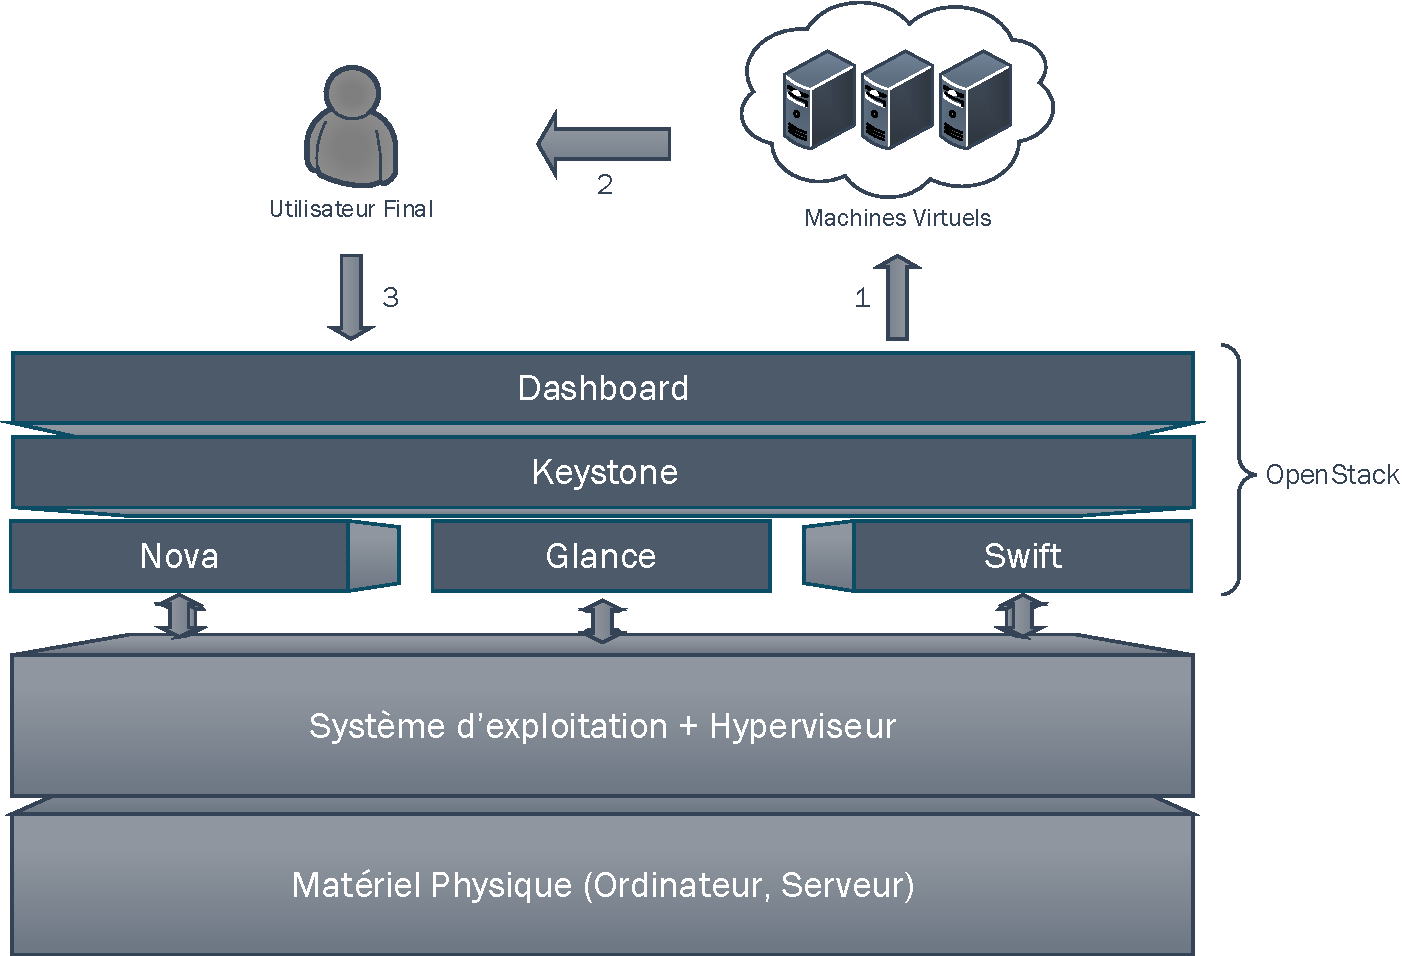
\includegraphics[scale=0.8,angle=90]{images/principeOpenStack-crop.pdf}
\end{center}
\section{Schémas global} \label{sch:glob}

\chapter{Scripts d'automatisation}
\section{Solaris}
\subsection{nataddrule.sh}
%\begin{minted}[frame=single,fontfamily=courier,linenos,mathescape]{bash}
%\end{minted}

\chapter{Fichiers de configuration OpenStack}
\section{Keystone}
\subsection{keystone.conf}

\section{Glance}

\section{Swift}

\section{Nova}

\chapter{Fichiers de configuration Solaris}
\section{NAT}
\subsection{ipf.conf} \label{conf:NAT}
\section{Reverse Apache} \label{conf:apacheProxy}

\chapter{Recettes Puppet}

\nocite{*}
\printbibliography

\deftranslation{Glossary}{Glossaire}
\printglossaries


% Le résumé
% Pas de glossaire dans le résumé
\begin{abstract}
Derrière le mot \gls{cloudcomputing} se trouvent de nombreux thèmes de l'informatique tels que la \gls{virtualisation}, la haute disponibilité, et la scalabilité.
La mise en place d'un \gls{cloudprive} est donc un sujet d'étude particulièrement intéressant en Réseaux \& Télécommunications.\newline
A l'aide d'\gls{openstack} nous avons mis en place une Infrastructure en tant que Service, ce qui nous as permis de mieux comprendre l'interaction entre les différents service (Réseau, Stockage, \Gls{virtualisation}).
L'installation a été effectué sur des systèmes UNIX (Solaris) et Linux (CentOS, Ubuntu Server) dont les choix sont expliqués dans ce rapport.\newline
En plus des services d'OpenStack nous avons intégrés une gestion de configuration automatique pour les instances virtuelles à l'aide de Puppet.
La mise en place de monitoring à l'aide de Shinken et Munin est également détaillé.\newline\newline

\noindent Behind what we call \gls{cloudcomputing} there is a bunch of interesting topics like virtualization, high-disponibility, and scalability.
This make deploying a Private Cloud an interesting studies subject in Networking \& Telecommunications.\newline
We used OpenStack, an open-source software, to create an Infrastructure as a Service, this gave us a better understanding of service's interaction (Networking, Storage, Virtualization).
Setup was made on both UNIX (Solaris) and Linux (CentOS, Ubuntu Server) systems whose choice are explained in this report.\newline
In additions of OpenStack services we used Puppet to deliver automated configuration deployment to VMs.
Monitoring with Shinken and Munin is also detailled.

\end{abstract}

\end{document}
